\documentclass{amsart}
\usepackage{graphicx}
\graphicspath{{./}}
\usepackage{hyperref}
\usepackage{csvsimple}
\usepackage{longtable}
\usepackage{epigraph}
\title{Human Race Important Things in Life By Ethnicity}
\author{Zulfikar Moinuddin Ahmed}
\date{\today}
\begin{document}
\maketitle

\section{Invariance of Distributions}

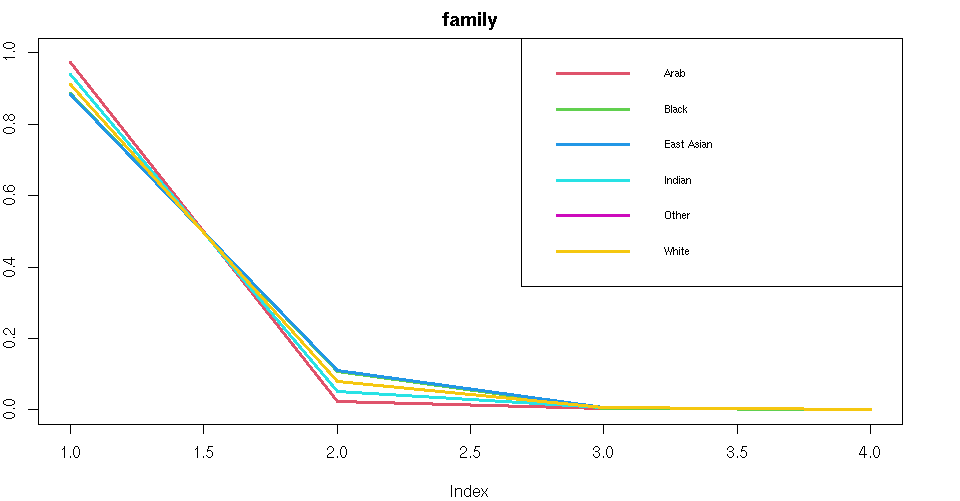
\includegraphics[scale=0.6]{ethfam.jpeg}

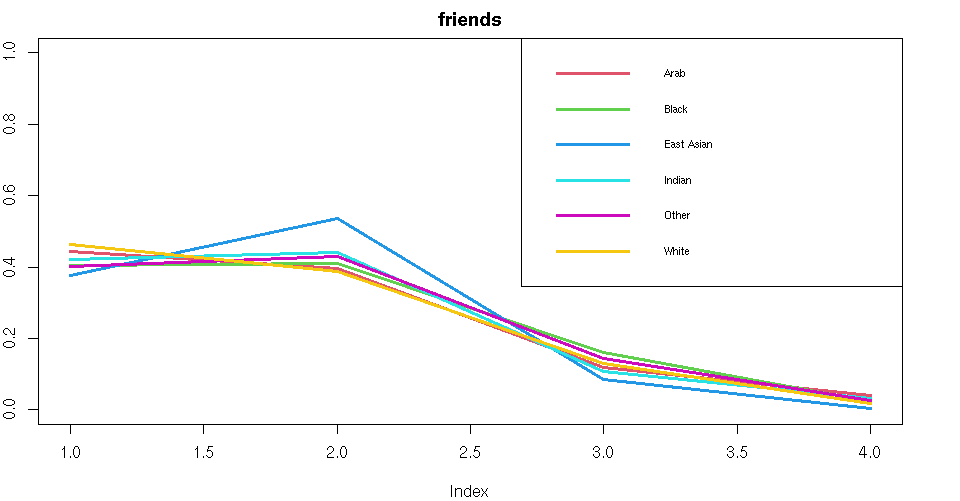
\includegraphics[scale=0.6]{ethfriends.jpeg}

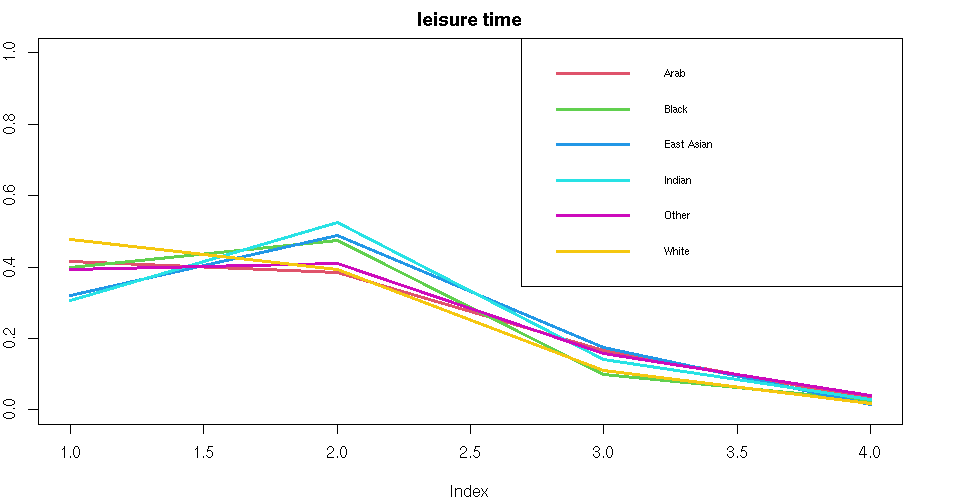
\includegraphics[scale=0.6]{ethleis.jpeg}

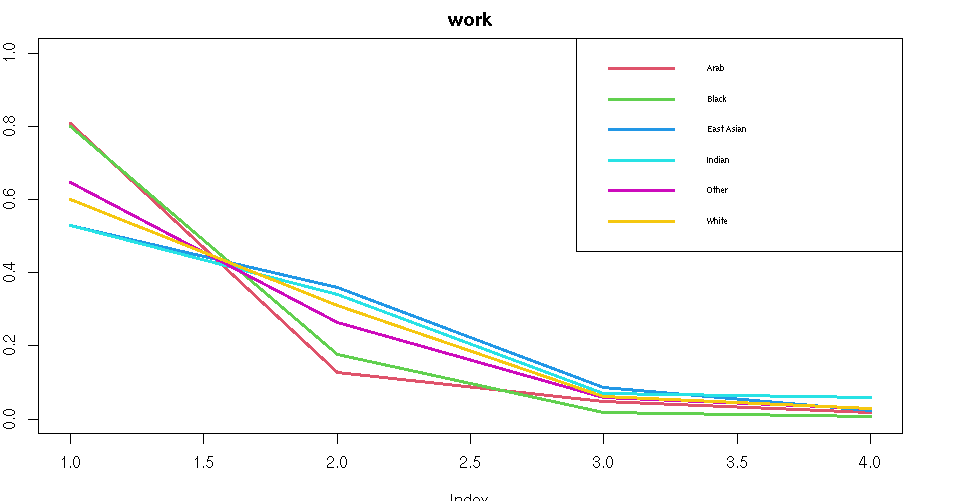
\includegraphics[scale=0.6]{ethwork.jpeg}

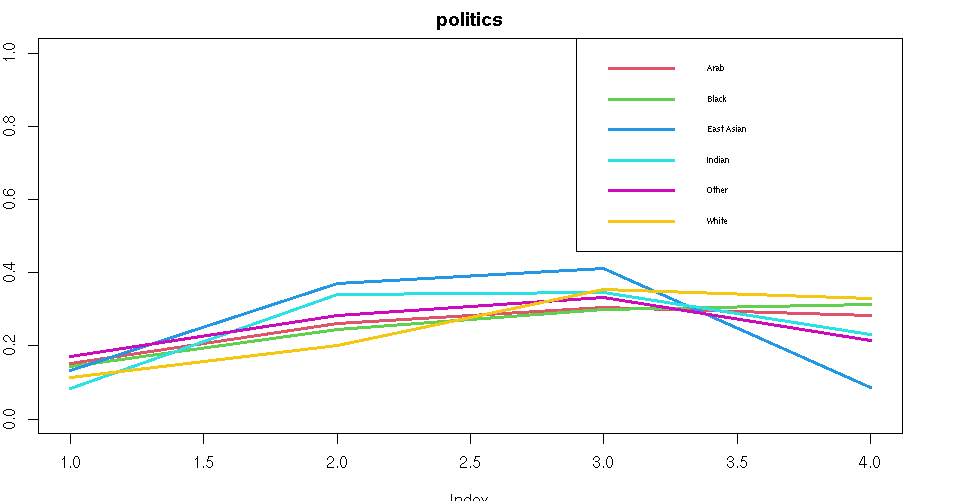
\includegraphics[scale=0.6]{ethpol.jpeg}

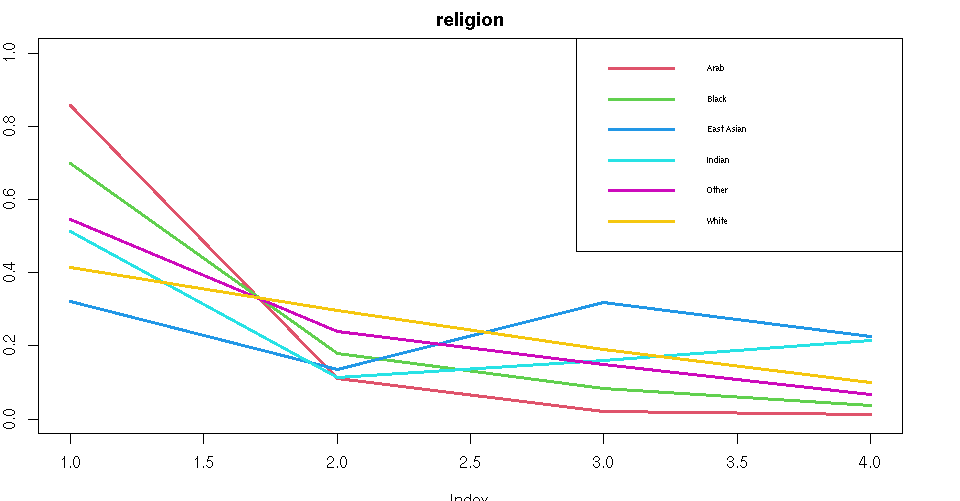
\includegraphics[scale=0.6]{ethrel.jpeg}

This gives you a visual feel for the regularity of six facets of life on Earth across ethnicities.


\section{Ethnicity Effects on Universal Human Preference Curve}

\subsection{Family}

Maximum effect 0.63\% of variation.

% latex table generated in R 4.0.3 by xtable 1.8-4 package
% Sun May  9 16:03:20 2021
\begin{table}[ht]
\centering
\begin{tabular}{rlr}
  \hline
 & eth & explained \\ 
  \hline
1 & Arab & 0.63 \\ 
  2 & Black & 0.27 \\ 
  3 & East Asian & 0.30 \\ 
  4 & Indian & 0.12 \\ 
  5 & Other & 0.01 \\ 
  6 & White & 0.01 \\ 
   \hline
\end{tabular}
\end{table}


\subsection{Friends}

Maximum ethnicity effect 1.08\% of variation.

% latex table generated in R 4.0.3 by xtable 1.8-4 package
% Sun May  9 16:07:11 2021
\begin{table}[ht]
\centering
\begin{tabular}{rlr}
  \hline
 & eth & explained \\ 
  \hline
1 & Arab & 0.65 \\ 
  2 & Black & 0.56 \\ 
  3 & East Asian & 3.35 \\ 
  4 & Indian & 0.11 \\ 
  5 & Other & 0.20 \\ 
  6 & White & 1.08 \\ 
   \hline
\end{tabular}
\end{table}

\pagebreak

\subsection{Leisure Time}

Maximum ethnicity effect 3.2\%.

% latex table generated in R 4.0.3 by xtable 1.8-4 package
% Sun May  9 16:07:51 2021
\begin{table}[ht]
\centering
\begin{tabular}{rlr}
  \hline
 & eth & explained \\ 
  \hline
1 & Arab & 1.51 \\ 
  2 & Black & 0.73 \\ 
  3 & East Asian & 1.97 \\ 
  4 & Indian & 3.17 \\ 
  5 & Other & 0.50 \\ 
  6 & White & 3.12 \\ 
   \hline
\end{tabular}
\end{table}


\subsection{Politics}

Maximum ethnicity effect 5.11\%

% latex table generated in R 4.0.3 by xtable 1.8-4 package
% Sun May  9 16:08:13 2021
\begin{table}[ht]
\centering
\begin{tabular}{rlr}
  \hline
 & eth & explained \\ 
  \hline
1 & Arab & 1.42 \\ 
  2 & Black & 3.15 \\ 
  3 & East Asian & 11.16 \\ 
  4 & Indian & 2.04 \\ 
  5 & Other & 0.85 \\ 
  6 & White & 5.11 \\ 
   \hline
\end{tabular}
\end{table}

\subsection{Work}

Maximum ethnicity effect 6.5\% of variation.

% latex table generated in R 4.0.3 by xtable 1.8-4 package
% Sun May  9 16:08:49 2021
\begin{table}[ht]
\centering
\begin{tabular}{rlr}
  \hline
 & eth & explained \\ 
  \hline
1 & Arab & 6.36 \\ 
  2 & Black & 4.68 \\ 
  3 & East Asian & 5.98 \\ 
  4 & Indian & 5.49 \\ 
  5 & Other & 0.01 \\ 
  6 & White & 1.09 \\ 
   \hline
\end{tabular}
\end{table}

\subsection{Religion}

This is one feature that has some significant ethnic effects up to 35\% of variation.

% latex table generated in R 4.0.3 by xtable 1.8-4 package
% Sun May  9 16:09:18 2021
\begin{table}[ht]
\centering
\begin{tabular}{rlr}
  \hline
 & eth & explained \\ 
  \hline
1 & Arab & 16.20 \\ 
  2 & Black & 5.60 \\ 
  3 & East Asian & 36.03 \\ 
  4 & Indian & 5.10 \\ 
  5 & Other & 1.45 \\ 
  6 & White & 11.77 \\ 
   \hline
\end{tabular}
\end{table}


\section{R Code}

\begin{verbatim}
pref.eth<-function(v){
  A<-rownrm(table(life[,c("eth",v)]))
  print(dim(A))
  eth<-row.names(A)
  
  mv <- colSums(A)/6.0
  A0 <- matrix( 0, nrow=6, ncol=4)
  for (r in 1:6){ A0[r,]<-mv }
  S <- A - A0
  explained.var<-rep(0,6)
  for (s in 1:6){
    explained.var[s]<-sum(S[s,]^2)/sum(A[s,]^2)
  }
  data.frame(eth=eth,explained=explained.var*100)
}


\end{verbatim}

\section{Conclusions}

There is some significant ethnicity effects for Religion,but for all others there is a minor ethnicity effect, which implies the case for Universal Human Nature for the mean distributions independent of ethnicity.

\end{document}
